\chapter{Motivation}\label{chp:motivation}


%===================================================================================================%
\section{Introduction}
%===================================================================================================%

Well, everbody needs some good motivation, aye?

%===================================================================================================%
\section{What is Serverless?}\label{sec:whatIsServerless}
%===================================================================================================%

"Serverless" is one of the most discussed technologies, prominently featured in many Gartner Hype-Cycle reports that identify trends and emerging technologies which they will think will shape the industries future. 
\autocite{Smith2017Hype2017}\highcomma
\autocite{Weiss2017Hype2017}\highcomma
\autocite{Natis2017Hype2017}\highcomma
\autocite{Walker2017Hype2017}\highcomma
\autocite{DawsonPhilip2017Hype2017}
Consequently, various definition attempts were made:


\begin{enumerate}
    \item \textbf{Roberts}\\
        "[Serverless refers to] custom code that's run in ephemeral containers (Function as a Service or "FaaS").[...] Such architectures remove the need for the traditional 'always on' server system sitting behind an application. Depending on the circumstances, such systems can significantly reduce operational cost and complexity."\autocite{Roberts2016ServerlessArchitectures}
    \item \textbf{Hammond, Rymer} \\
        "Serverless is an approach to development that removes their need to care about servers: provisioning, setting up, configuring, or otherwise interacting with them. Beyond that, the name connotes a new architectural approach and operating principles. A serverless architecture encompasses multiple development services, the most notable of which are FaaS offerings like Amazon lambda, Google cloud Functions, Microsoft Azure Functions, and the Fx, OpenWhisk, and Riff open source projects.\\
        These services share four core elements. They: Support deployment of arbitrary business logic [...], Decouple state and compute [...], Automatically invoke and scale deployed logic [...], Support event sources and sinks [...]"\autocite{Hammond2018DemystifyingComputing}
    \item \textbf{Johnston}\\
        "A Serverless solution is one that costs you nothing to run if nobody is using it (excluding data storage). [...] So you would be paying for the storage of data, but not for idling servers.
        While the system is always available, it’s not always “on”.
        [...]
        Serverless isn’t (and never was) about “no servers”, at least not in the way that we would think about it.
        Serverless isn’t about just scalability.
        Serverless isn’t about Functions (FaaS) only, because you can always run non-Serverless elements and then pay for idle.
        A Serverless system such as this would be very low on maintenance too and is inherently event driven. If it wasn’t event-driven, then you’d need to pay to ensure that a system is always available and idle (like an EC2 instance)"\autocite{Johnston2017AServerless}
    \item \textbf{Kehoe}\\
        "Like so many things in life, serverless is not an all-or-nothing proposition. It’s a spectrum — and more than that, it has multiple dimensions along which the degree of serverlessness can vary.
        For a service to be “more serverless”, it needs to move in one or more of the following directions:
        \begin{enumerate}[nolistsep]
            \item Service-full + ephemeral compute
            \item Tighter correspondence between resources used and resources billed
            \item Smaller and more abstracted control plane
        \end{enumerate}
        [...] Serverless is, at a functional level, about lower operations burden and faster time to market."\autocite{Kehoe2017TheSpectrum}
    \item \textbf{Castro et. al.}\\\label{castro}
        "[Serverless is] a cloud-native platform 
        for
        short-running, stateless computation
        and
        event-driven applications
        which 
        scales up and down instantly and automatically
        and
        charges for actual usage at a millisecond granularity"\autocite{Castro2017ServerlessService}
    \item \textbf{Amazon Web Services}\\
        "Serverless computing allows you to build and run applications and services without thinking about servers. Serverless applications don't require you to provision, scale, and manage any servers. You can build them for nearly any type of application or backend service, and everything required to run and scale your application with high availability is handled for you."\autocite{AmazonWebServices2017ServerlessServices}
    \item \textbf{Microsoft Azure}\\
        "Serverless computing is the abstraction of servers, infrastructure, and operating systems. When you build serverless apps you don’t need to provision and manage any servers, so you can take your mind off infrastructure concerns. Serverless computing is driven by the reaction to events and triggers happening in near-real-time—in the cloud. As a fully managed service, server management and capacity planning are invisible to the developer and billing is based just on resources consumed or the actual time your code is running."\autocite{MicrosoftAzure2017ServerlessAzure}
    \item \textbf{serverless.com}\\
        "The serverless movement started with the release of AWS Lambda, a Function-as-a-Service (FaaS) compute service. But serverless is much more than just FaaS.\\
        Ultimately, serverless is about focusing your efforts on what provides value to your users. This means using managed services for databases, search indexes, queues, SMS messaging, and email delivery. It means tying these services together using stateless, ephemeral compute like the various FaaS offerings."\autocite{ServerlessTeam2017WhyServerless}
\end{enumerate}

In context of this study, Mike Roberts' definition will be used as a foundation to understand the topic since it is the most universally applicable and open description among the options. Other definition attempts, such as \textbf{Hammod and Rymer}, will be used to discuss serverless system properties in depth.

To understand this very broad definition of "serverless", the first step is to understand what a server is and how a serverless system differs from it. \textquote{A server is a computer designed to process requests and deliver data to another computer over the internet or a local network}\autocite{Mitchell.Bradley2018TheServer}, meaning that a server poses as an accessible endpoint that waits for requests from clients and responds to them. It is \textit{continuously} running, even if there is no task to be processed in order to be ready for incoming requests. This waiting-time is called 'idle time' and presents the most significant difference between servers and serverless systems: while the server waits for incoming requests to process them, in a serverless context a computational unit is created for every incoming request.

\begin{figure}[ht]
    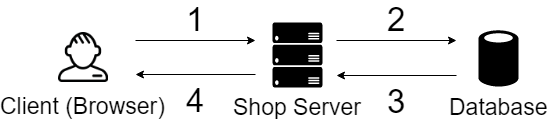
\includegraphics[width=0.9\linewidth]{images/drawio/3tier-oneclient.png}\centering
    \caption {Classic Three-Tier Architecture}
    \label{fig:3tier1client}
\end{figure}

Figure \ref{fig:3tier1client} presents this structure using the example of an online shop. It depicts the classic three-tier-model that consists of the presentation (client), logic (server) and data (database) tier.\autocite{Ramirez2000Three-TierArchitecture} In a situation where a customer intends to purchase an item, first, the client sends a request to the shop's server, which will process it by querying the database for the amount of items in stock, performing the purchase (writing to the database) and lastly responding to the client whether his request was successful or not. More abstract speaking, the action of buying one item is realized as a sequence of a finite amount of steps that have to be passed in order to achieve the desired result. This workflow is the same for each request, but what happens if multiple customers want to $buy$ an item simultaneously? \\
% As illustrated in Figure \ref{fig:3tierNclient}, the amount of steps that have to be performed concurrently to process every request in a timely manner grows with every added client. \\
% \begin{figure}[ht]
%     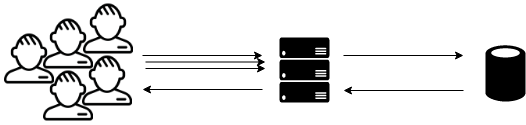
\includegraphics[width=0.9\linewidth]{images/drawio/3tier-multipleclient.png}\centering
%     \caption {Classic Three-Tier Architecture with multiple Clients}
%     \label{fig:3tierNclient}
% \end{figure}
The amount of steps that have to be performed concurrently to process every request in a timely manner grows with every added client but since a server operates on a finite amount of resources, eventually a performance-wise degradation of service occurs. Traditionally, more servers and therefore more available computing power would be added to a system to cope with this challenge. However, this approach results in a very inflexible provision of resources which is illustrated in Figure \ref{graph:provisionedComputePowerServer} on page \pageref{graph:provisionedComputePowerServer}. To further support this hypothesis, the following example assumes that each server can handle exactly 1000 clients. If 1001 clients simultaneously connect to the system, at least two servers have to be running to satisfy the calls. This directly means that it is never possible to accurately provision just the right amount of processing power for the incoming request but either too much or not enough. 

\begin{figure}[ht]
    \begin{tikzpicture}
        \begin{axis}[
                ,xlabel         = $\# Requests$
                ,ylabel         = {$Provisioned \, Compute \, Power$}
                ,yticklabels    = {,,}
                ,xticklabels    = {,,}
                ,axis x line    = bottom
                ,axis y line    = left
                ,domain         = 0:6
                ,ymajorgrids    = true
                ,grid style     = dashed
                ]
            \addplot [const plot, no marks, color=blue] coordinates {(0,1) (1,2) (2,3) (3,4) (4,5) (5,6)};
            \addplot [color=white]{x};
        \end{axis}
    \end{tikzpicture}\centering
    \caption {Provisioned Compute Power: Server Model}
    \label{graph:provisionedComputePowerServer}
\end{figure}

Comparatively in a serverless approach, the function that executes the steps necessary to fulfill the request is initiated with its own small runtime. How this works from a technical perspective is discussed later on in chapter \ref{sec:serverless} on page \pageref{sec:serverless}. A drastically simplified sketch of this approach can be seen in Figure \ref{fig:serverlessArchHighlevel}. The gateway is an API endpoint that reroutes incoming requests to a server, or in this case to a serverless function that is in turn instantiated. \autocite{Kelly2010UsingInvalidation} This gateway distributes the calls to the newly spun-up functions which is called "fan-out"\autocite{Do2013Limplock}, a term that describes how the system structure fans out after the gateway. 

\begin{figure}[ht]
    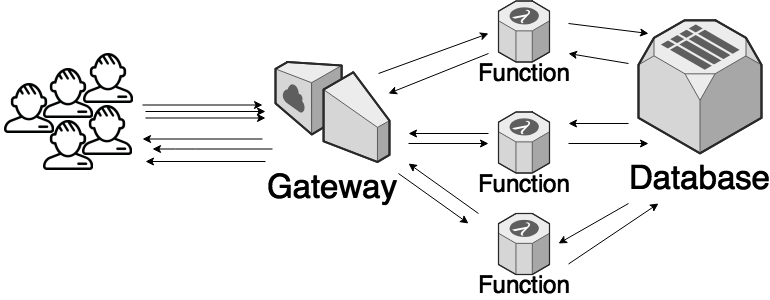
\includegraphics[width=\linewidth]{images/drawio/lambda.png}\centering
    \caption {Serverless Architecture (simplified)}
    \label{fig:serverlessArchHighlevel}
\end{figure}

Since the amount of running functions is directly proportional to the number of incoming requests, the system always provisions the exact processing power needed to sufficiently handle the load. In comparison, a serverless strategy is more efficient, which can be seen in Figure \ref{graph:provisionedComputePowerComparison}.

\begin{figure}[ht]
    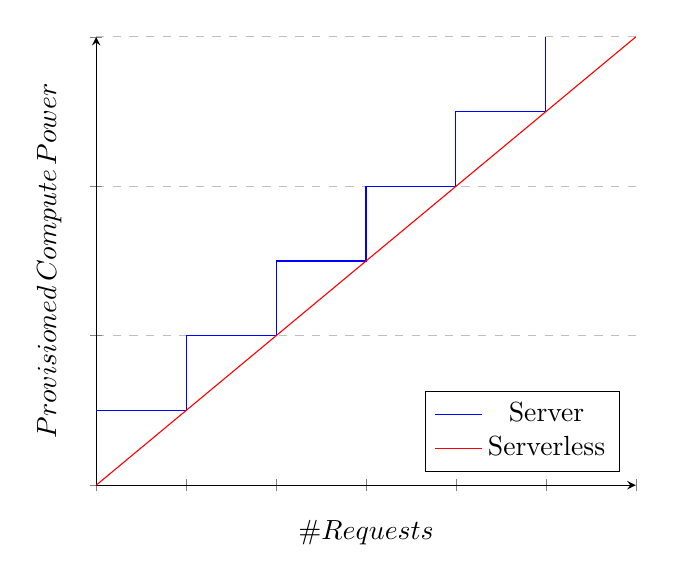
\begin{tikzpicture}
        \begin{axis}[
                ,xlabel         = $\# Requests$
                ,ylabel         = {$Provisioned \, Compute \, Power$}
                ,yticklabels    = {,,}
                ,xticklabels    = {,,}
                ,axis x line    = bottom
                ,axis y line    = left
                ,domain         = 0:6
                ,legend pos     = south east
                ,ymajorgrids    = true
                ,grid style     = dashed
                ]
            \addplot [const plot, no marks, color=blue] coordinates {(0,1) (1,2) (2,3) (3,4) (4,5) (5,6)};
            \addlegendentry{Server}
            \addplot [color=red]{x};
            \addlegendentry{Serverless}
        \end{axis}
    \end{tikzpicture}\centering
    \caption {Provisioned Compute Power Comparison: Server/Serverless}
    \label{graph:provisionedComputePowerComparison}
\end{figure}

%===================================================================================================%
\section{Why Serverless?}
%===================================================================================================%

In recent years \acf{IoT} has been one of the major growth markets and is expected to reach a global revenue of \$457B by the end of 2020\autocite{Columbus20172017Forecasts}, attaining a \acf{CAGR} of 28.5\% over four years.\autocite{Columbus20172017Forecasts} Looking at the most common use cases for IoT applications, it is clear that the prevailing real-life scenarios can be characterized by ubiquitous sensors numbering in the millions or even billions constantly monitoring physical objects, events and humans alike. Right now, these observations are often communicated to a cloud data center for various analyses that in turn trigger reactions to the observed events which aims to improve the efficiency and reliability of the systems and generate valuable insights.\autocite{Yannuzzi2014KeyComputing} \\
This pattern results in a closed-loop \acf{OODA} cycle, where the three major components of the information-processing-system are the information \textit{producers} (sensors), the \textit{cloud endpoint} and the \textit{consumer} or \textit{processor}.\autocite{Shukla2017BenchmarkingApplications} Especially this closed-loop characteristic of IoT applications is essential for their effective use and seamless communication between observing events and processing them is therefore a fundamental requirement. To derive actionable insights that have a business impact it is essential to process the data ingress in near real-time since information often has a time-to-live and are only valid for a short amount of time, hence a rapidly scaling processor-concept that is performant enough to digest the data ingress is an imperative system component. \acf{ESP} approaches are an obvious solution to this challenge and all reference IoT solutions from cloud providers \footnote{\url{https://aws.amazon.com/iot-core/features/}}\textsuperscript{,}\footnote{\url{https://microsoft.com/en-in/cloud-platform}} include some element of event streaming.

%===================================================================================================%
\section{Scientific Body of Knowledge}
%===================================================================================================% 

Academically speaking, serverless \textit{computing} architectures have been a topic of interest for a short period of time. The vast majority of research, however, is focusing on defining the technology and is content with describing and characterizing it. Six particularly important\footnote{based on the number of citations and publisher impact factor (Scimago Journal \& Country Rank)} scientific publications are especially noteworthy:

\begin{enumerate}
    \item 
        \textbf{Baldini et. al.} describe "serverless" as \blockquote{a set of stateless functions, along with the events that should trigger their activation [and] a serverless runtime [that] allocates resources as events arrive, avoiding the need for costly pre-allocated or dedicated hardware.} They discuss the challenges that emerge when programming a composition of functions, where the composition is a serverless function itself. Moreover, they identify three main constraints for composing functions: First, functions should be considered as black boxes, secondly, function composition should obey a substitution principle with respect to synchronous invocation and third,  invocations should not be billed more than once. As a result, they demonstrate an addition to the core of an open-source serverless runtime that enables composition of functions that satisfies all three constraints.\autocite{Baldini2017TheComputing}
    \item
        \textbf{McGrath and Brenner} discuss the design, implementation and operation of a performance-oriented serverless computing platform that is implemented in .NET that utilizes Windows containers as function execution environments and is deployed on Microsoft Azure. They focus on implementation obstacles such as scaling and container recovery. Furthermore, they propose metrics to measure the performance of serverless platforms like AWS Lambda, Azure Functions, Google Cloud Functions and Apache OpenWhisk and compare their prototypical function to the test results from commercial serverless platforms. Overall, they observe a higher throughput with their prototype in comparison.\autocite{McGrath2017ServerlessPerformance}
    \item 
        \textbf{Nastic et. al.} apply the serverless architecture pattern to edge-data analytics use-case. They present a \textquote{novel approach [that] implements cloud-supported, real-time data analytics in edge-computing applications}. Main focus of the study is to introduce an application model and to examine main design requirements and challenges based on real-life healthcare scenarios.\autocite{Nastic2017AComputing}
    \item 
        \textbf{Malawski et. el.} focus on the specific use case of scientific workflows. In a research context, they introduce the academic field of experiments as a complex and important environment for computation approaches. Despite the commonly advertised use of serverless functions as background task runner for Web applications, Malawski et. al. evaluate their applicability on compute- and dataintensive workloads. Using Google Cloud Functions coupled with the HyperFlow workflow engine, the team present a prototype that is capable of running as a task on the Google Cloud Infrastructure, staging data to and from Cloud storage and can execute custom application binaries. The study concludes that the prototype is indeed suited for scientific workloads, demonstrated with the Montage\footnote{\url{http://montage.ipac.caltech.edu/}} astronomic workflow.\autocite{Malawski2017ServerlessFunctions}
    \item 
        \textbf{Castro et. al.} identify key characteristics and use cases of serverless architectures. In addition, they describe technical challenges and discuss problems that can occur in various environments.
    \item
        \textbf{Bila et. al.} explore the design of an automated thread mitigation system based on a serverless architecture. They argue that the typical mitigation workflow is inherent event-driven and is therefore a great fit to be implemented in a serverless architecture.  \autocite{Bila2017LeveragingContainers}
\end{enumerate}

Interestingly, all of the above mentioned studies share some common characteristics: they focus on \textit{how} to implement serverless architectures or \textit{what} it is, but do not conduct any extensive comparative analysis aiming to directly study the differences to other architectural patterns. Equally striking is the fact, that every study was published in 2017 or 2018 although the first widespread public service offering serverless computing, AWS (Amazon Web Services) Lambda, was introduced back in 2014.\autocite{Lindblom2014AWSBlog}

Apart from these scientific studies, there are a few other publications worth mentioning. To begin with, Stigler gave an introduction to the topic by aiming to "understand exactly what serverless computing is, how it works and the benefits and use cases for serverless computing". She gives hands-on examples for AWS Lambda and Azure Functions.\autocite{Stigler2018UnderstandingComputing}\\
Similar to other trends in technology, there are thousands of blog articles that address the topic. One of the most discussed and recognized posts is "\textit{Serverless Architectures}" by Mike Robert on the popular blog \url{martinfowler.com}\autocite{Roberts2016ServerlessArchitectures}. He tackles the question "What is Serverless?" and discusses advantages and drawbacks. \\
In addition to these non-scientific publications, there are proprietary market research reports from institutions like Gartner
\autocite{Smith2017Hype2017}\highcomma
\autocite{Weiss2017Hype2017}\highcomma
\autocite{Natis2017Hype2017}\highcomma
\autocite{Walker2017Hype2017}\highcomma
\autocite{DawsonPhilip2017Hype2017}
and Forrester\autocite{Hammond2018DemystifyingComputing}. These reports often lack the disclosure of used research methods and are therefore hard to use as the sole foundation for a scientific recommendation. 

To conclude, there have been several scientific publications in the recent twelve months that try to define the concept of serverless computing architectures and numerous non-scientific writings on the topic. For the vast majority of studies, the researchers were unambiguously focused on examining the technology as an isolated phenomenon. The existing scientific body of knowledge and the academic understanding of the topic will be further examined in chapter \ref{sec:serverless}.

%===================================================================================================%
\section{Research Objective}
%===================================================================================================%

The purpose of this research is to evaluate the suitability and viability of the serverless architecture pattern by comparing it in a prototypical scenario. The result will be a simplified decision-framework for architects that enables them to decide if a "serverless" architectural approach is fitted for their stream-processing use-case.

One sub-objective is to assess the current industry understanding of "serverless" and evaluate the suitability and viability of this architecture pattern.
Moreover, it is supposed to assist the process of high-level system design by providing a reference and guidance by introducing fPaaS\footnote{"Function-Platform-as-a-Service". Defined by Gartner \autocite{Chandrasekaran2017EvolutionWhen}} capabilities and caveats.\\
An important aspect is to discuss not only the advantages of the serverless architecture pattern but also to evaluate the caveats and shortcomings of said architecture and its impact. To provide the reader with a comprehensive view on the subject, it is additionally the goal of this research to characterize the design compromises that have to be made when applying the serverless approach.  

%===================================================================================================%
\section{Summary}
%===================================================================================================%

The serverless computing architecture pattern is a very interesting and novel approach to existing problems and challenges. In the recent twelve months, there have been several scientific publications that try to define the concept of serverless compute architectures and numerous non-scientific writings on the topic have been published too. The vast majority, however, does not compare this architecture approach to traditional alternatives under scientific test conditions. \\
It is therefore this study's objective to evaluate the suitability and viability of the serverless architecture pattern by comparing it in a prototypical scenario. As a result, a simplified decision-framework for architects that enables them to decide if a "serverless" architectural approach is fitted for their stream-processing use-case will be presented. Furthermore, caveats and shortcomings of said architecture and its impact will be discussed. 
In order to do so, the existing scientific body of knowledge and the academic understanding of the topic will be further examined in the following chapter and the reader's specific domain knowledge will be elevated (TODO: besseres Wort). 